\documentclass{beamer}

\usepackage{alltt}%
\usetheme{Boadilla}
\usecolortheme{seahorse}

%\usepackage{listings}
\makeatletter
\def\maxwidth{ %
  \ifdim\Gin@nat@width>\linewidth
    \linewidth
  \else
    \Gin@nat@width
  \fi
}
\makeatother

\definecolor{fgcolor}{rgb}{0.345, 0.345, 0.345}
\newcommand{\hlnum}[1]{\textcolor[rgb]{0.686,0.059,0.569}{#1}}%
\newcommand{\hlstr}[1]{\textcolor[rgb]{0.192,0.494,0.8}{#1}}%
\newcommand{\hlcom}[1]{\textcolor[rgb]{0.678,0.584,0.686}{\textit{#1}}}%
\newcommand{\hlopt}[1]{\textcolor[rgb]{0,0,0}{#1}}%
\newcommand{\hlstd}[1]{\textcolor[rgb]{0.345,0.345,0.345}{#1}}%
\newcommand{\hlkwa}[1]{\textcolor[rgb]{0.161,0.373,0.58}{\textbf{#1}}}%
\newcommand{\hlkwb}[1]{\textcolor[rgb]{0.69,0.353,0.396}{#1}}%
\newcommand{\hlkwc}[1]{\textcolor[rgb]{0.333,0.667,0.333}{#1}}%
\newcommand{\hlkwd}[1]{\textcolor[rgb]{0.737,0.353,0.396}{\textbf{#1}}}%
\let\hlipl\hlkwb

\usepackage{framed}
\makeatletter
\newenvironment{kframe}{%
 \def\at@end@of@kframe{}%
 \ifinner\ifhmode%
  \def\at@end@of@kframe{\end{minipage}}%
  \begin{minipage}{\columnwidth}%
 \fi\fi%
 \def\FrameCommand##1{\hskip\@totalleftmargin \hskip-\fboxsep
 \colorbox{shadecolor}{##1}\hskip-\fboxsep
     % There is no \\@totalrightmargin, so:
     \hskip-\linewidth \hskip-\@totalleftmargin \hskip\columnwidth}%
 \MakeFramed {\advance\hsize-\width
   \@totalleftmargin\z@ \linewidth\hsize
   \@setminipage}}%
 {\par\unskip\endMakeFramed%
 \at@end@of@kframe}
\makeatother

\definecolor{shadecolor}{rgb}{.97, .97, .97}
\definecolor{messagecolor}{rgb}{0, 0, 0}
\definecolor{warningcolor}{rgb}{1, 0, 1}
\definecolor{errorcolor}{rgb}{1, 0, 0}
\newenvironment{knitrout}{}{} % an empty environment to be redefined in TeX


\usepackage[utf8]{inputenc}
\usepackage{default}

\usepackage{xcolor}%for color mixing

\usepackage{amsmath}%
\usepackage{amsfonts}%
\usepackage{amssymb}%
\usepackage{graphicx}

\usepackage{tikz}
\usepackage{multirow}
\usepackage{booktabs}

\setbeamertemplate{itemize/enumerate body begin}{\small}

%%%%%%%%%%%%%%%%%%%%%%%%%%%%%%%%%%%%%%%%%%%%%%%%%%%%%%%%%%%%%%%%%%%%%%%%%%%%%%%%%%

\title{Statistical Modelling: Beyond Linear Models, Generalized Linear Models}
\subtitle{Chapter 5}
\author{Timoth\'ee Bonnet}
\date{\today}

\begin{document}

%\lstset{language=R}%code

\AtBeginSection[]
{
  \begin{frame}<beamer>
    \frametitle{}
    \tableofcontents[currentsection,sectionstyle=show/show,subsectionstyle=show/shaded/hide]% down vote\tableofcontents[currentsection,currentsubsection,hideothersubsections,sectionstyle=show/hide,subsectionstyle=show/shaded/hide] 
  \end{frame}
}


\begin{frame}{}
\maketitle

\end{frame}
%%%%%%%%%%%%%%%%%%%%%%%

\begin{frame}{Simple linear models}
  \textbf{{\color{purple}{Response}} = {\color{blue}{Intercept}} + {\color{red}{Slope}} $\times$ {\color{orange}{Predictor}} + {\color{gray}{Error}}} \\

\centering
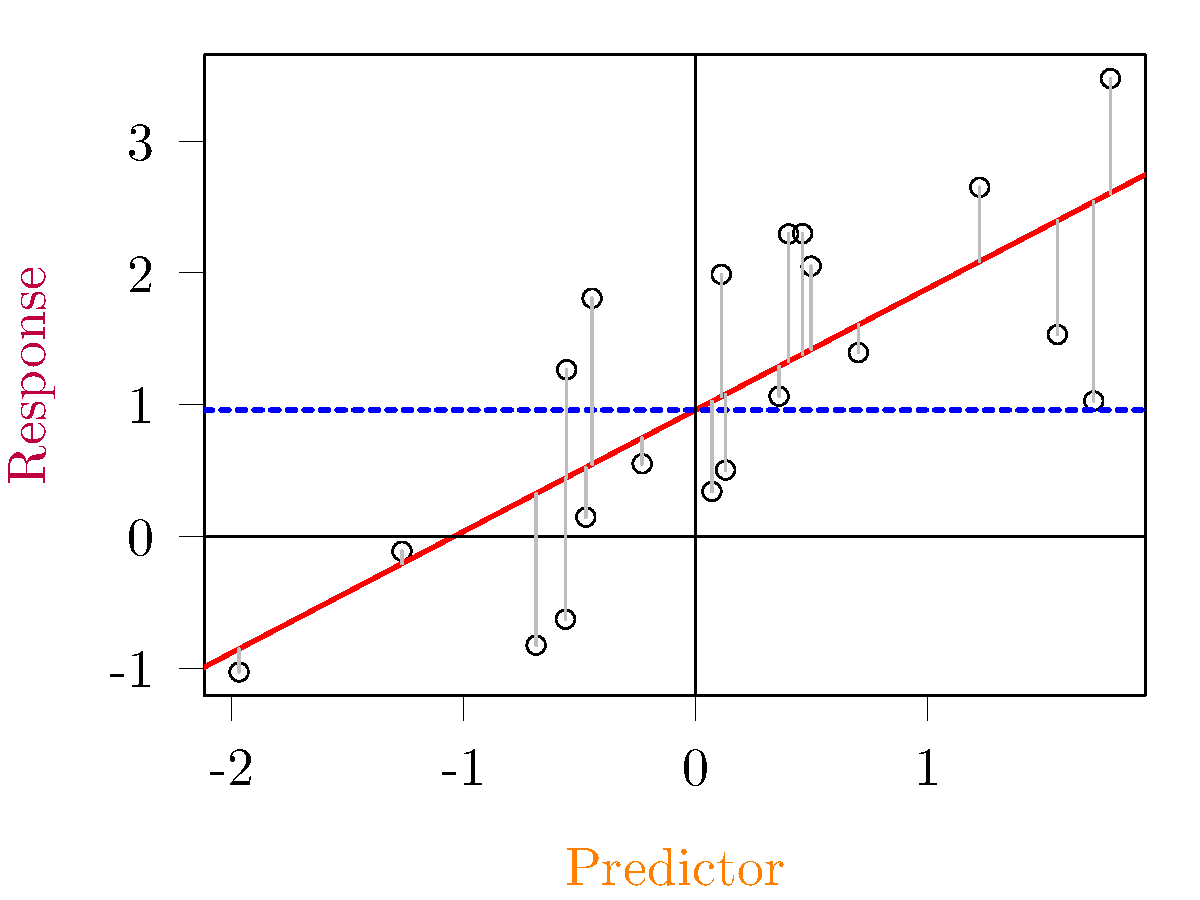
\includegraphics[width=0.6\textwidth]{Figures/figure/lmprinc-1}
\end{frame}
%%%%%%%%%%%%


\begin{frame}{Linear model basic assumptions}
 \begin{block}{}
     \begin{itemize}
      \item Predictor not perfectly correlated \\ \textit{Risk: Model won't run, unstable convergence, or huge SE}
       \item {\color{red!20!black}{Little error in predictors}}\\ \textit{Risk: bias estimates (underestimate with Gaussian error)}
       \item {\color{red!50!black}{Gaussian error distribution}}\\ \textit{Risk: Poor predictions}
       \item {\color{red!70!black}{Homoscedasticity (constant error variance)}}\\ \textit{Risk: Over-optimistic uncertainty, unreliable predictions}
       \item {\color{red!99!black}{Independence of error}}\\ \textit{Risk: Bias and over-optimistic uncertainty}
     \end{itemize}
 \end{block}
\end{frame}
%%%%%%%%%%%%


\begin{frame}{A simple linear model failure: binary data}

\centering
\only<1>{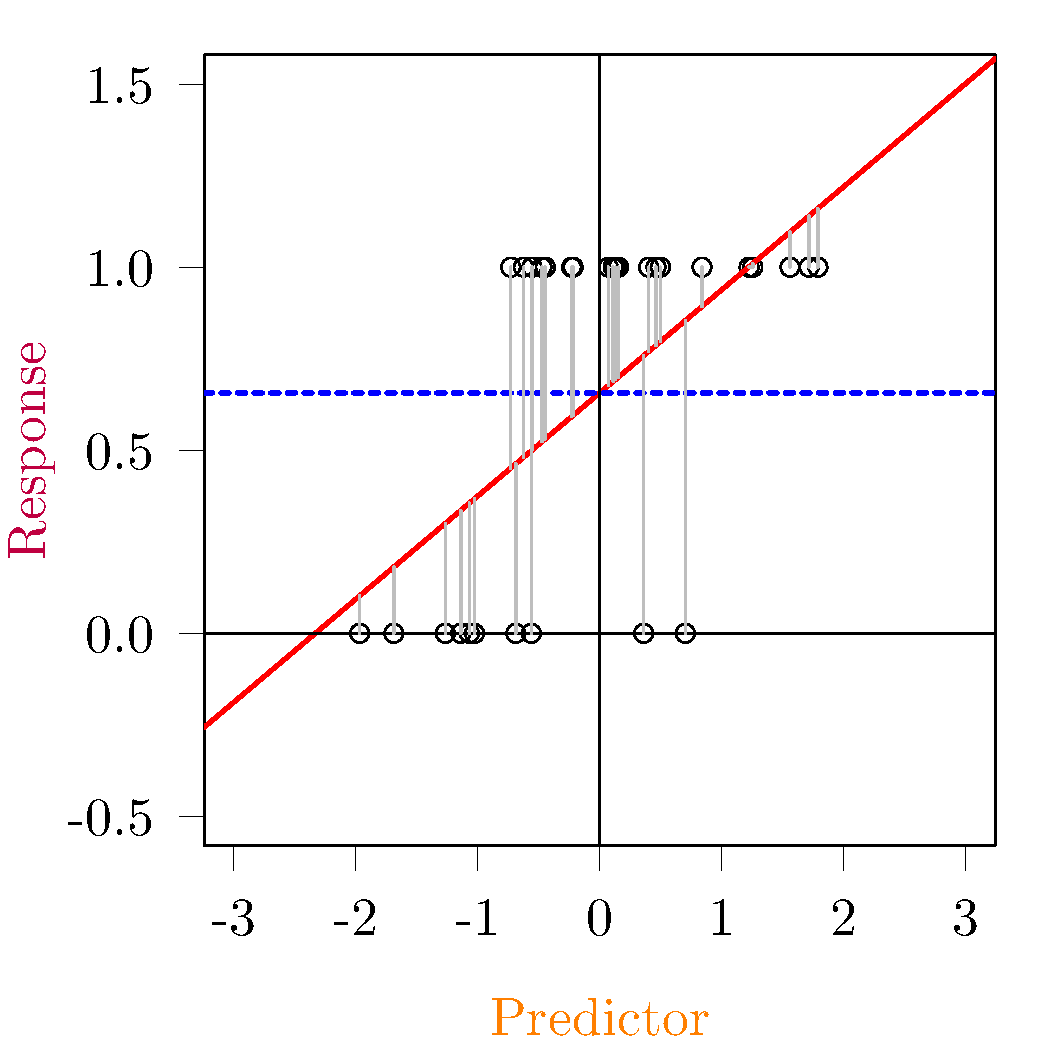
\includegraphics[width=0.6\textwidth]{Figures/figure/binlmprinc-1}}
\only<2>{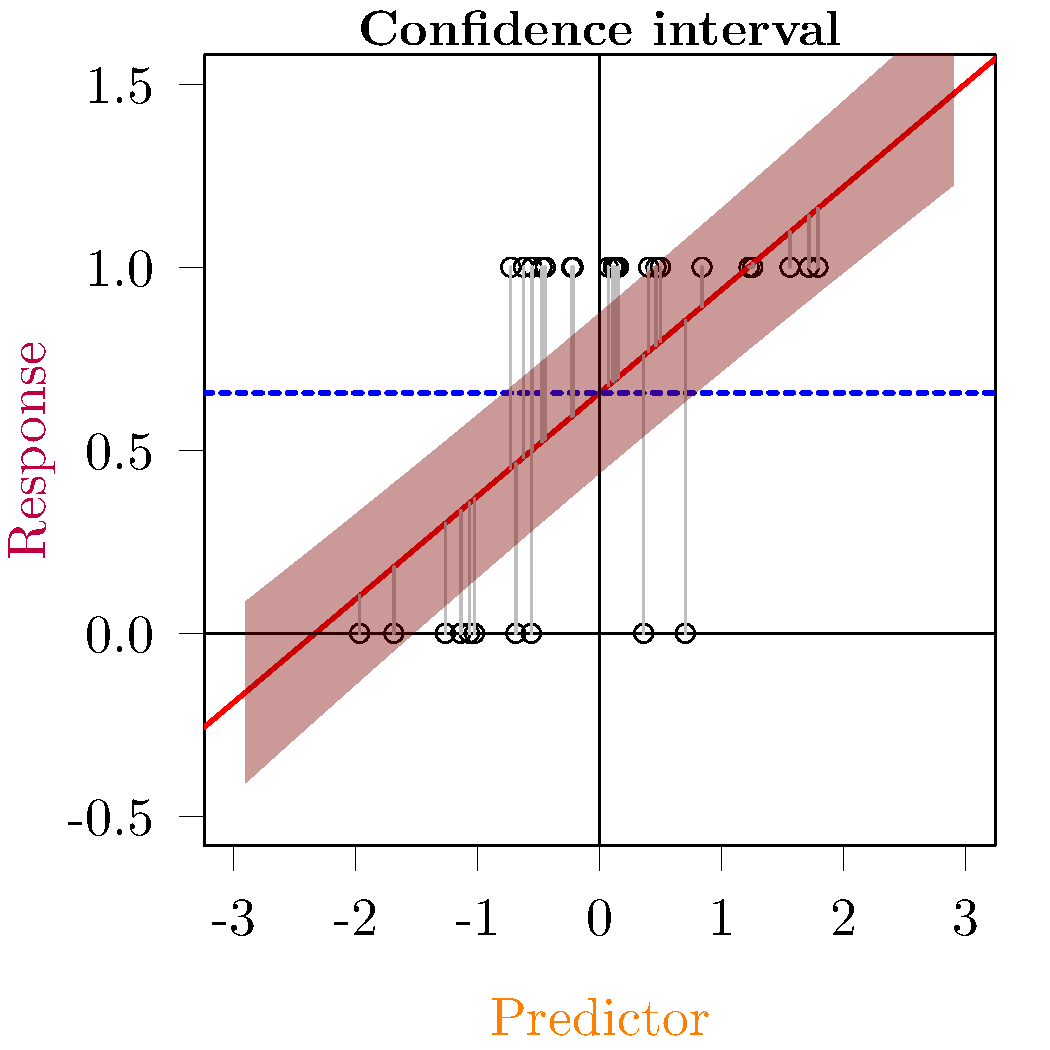
\includegraphics[width=0.6\textwidth]{Figures/figure/binlmprinc3-1}

  \begin{alertblock}{Assumptions violated:}
    Non-Gaussian errors, non-constant error variance, correlated errors
  \end{alertblock}
  }


\end{frame}
%%%%%%%%%%%%%

\begin{frame}{What we want our model to do}
\centering
 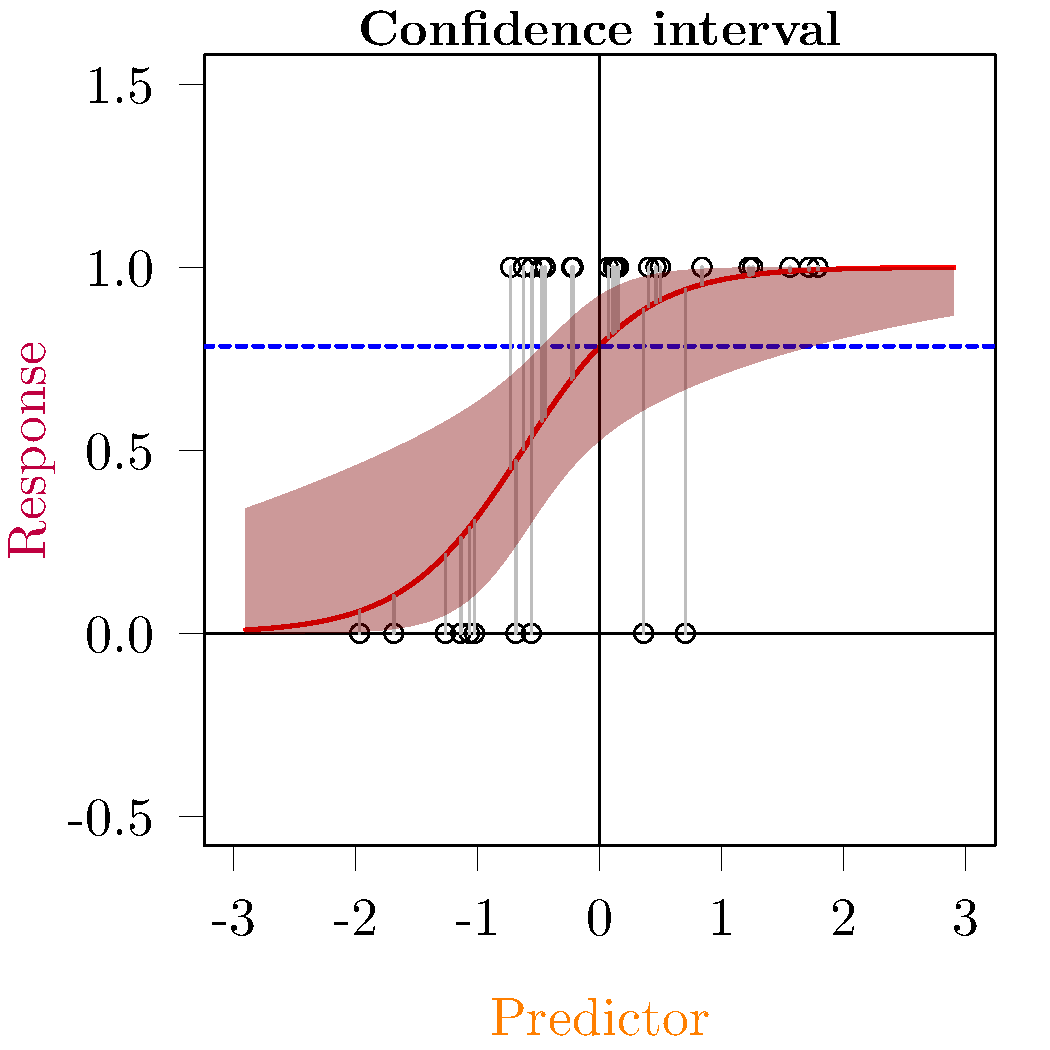
\includegraphics[width=0.6\textwidth]{Figures/figure/binglmprinc-1}
\end{frame}
%%%%%%%%%%%%


\begin{frame}{That is what a Generalized Linear Model does}

\begin{block}{Vocabulary warning}
  \begin{itemize}
    \item General Linear Model (=linear model with several responses, multivariate)
    \item \textbf{Generalized Linear Model (=non-normal errors, and uncertainty dependent on the mean)} 
  \end{itemize}
\end{block}

\pause

\begin{block}{What a GLM is:}
  \begin{enumerate}
    \item A linear function ($y = \mu + \beta x$ \dots)
    \item A probability distribution (Bernouilli, Binomial, Poisson\dots)
    \item A "link function" to convert between the scale of the linear function ($-\infty$ to $+\infty$) and the scale of the data and the probability distribution (often positive integer: 0, 1, 2, 3\dots)
  \end{enumerate}
  A GLM fits a continuous expected response; we observe discrete realizations
\end{block}

\end{frame}
%%%%%%%%%%%


\section{Binary data}

\begin{frame}{Logistic regression}

  \begin{block}{}
   
\begin{itemize}[<+->]
    \item Binary or proportion data (survival, presence/absence\dots)
    \item Binomial probability distribution ( = Bernouilly if binary data)
    \item Link function often logit: $y=\log(\frac{probability}{1-probability})$
    \item Back-transformation inverse-logit: $probability = \frac{1}{1 + exp(-y)}$
    \item Linear function $y = intercept + slope_1 predictor_1 + slope_2 predictor_2 +$
    \item For a given predicted $y$, $\exp(y)$ is the odd ratio: probability success / probability failure
  \end{itemize}
  
  
  \end{block}

  \end{frame}
  %%%%%%%%%%%%
  
\begin{frame}[fragile]{What is the Bernouilli distribution?}

    
\begin{knitrout}
\definecolor{shadecolor}{rgb}{0.969, 0.969, 0.969}\color{fgcolor}\begin{kframe}
\begin{verbatim}
bernouilli_random_sample <- rbinom(n = 10000, size = 1, prob = 0.3)
hist(bernouilli_random_sample)
mean(bernouilli_random_sample); 0.3
var(bernouilli_random_sample); 0.3*(1-0.3)
\end{verbatim}
\end{kframe}
\end{knitrout}

\end{frame}
%%%%%%%%%%%%

  
\begin{frame}[fragile]{Logistic regression in R}

    
\begin{knitrout}
\definecolor{shadecolor}{rgb}{0.969, 0.969, 0.969}\color{fgcolor}\begin{kframe}
\begin{verbatim}
glm(formula = obs ~ 1 + x, family = "binomial", data=data)
\end{verbatim}
\end{kframe}
\end{knitrout}

\end{frame}
%%%%%%%%%%%%

\begin{frame}{Does survival probability depend on size?}
 
  \begin{exampleblock}{Exercise, part 1}
    \begin{enumerate}
      \item Load \texttt{survivalsize.csv}
      \item Plot survival data. What kind of distribution is it?
      \item Fit a linear model and a logistic model with intercept only. How to interpret the estimates?
    \end{enumerate}
  \end{exampleblock}
  
  \pause
  
  \begin{block}{hints:}
  \begin{enumerate}
   \item For a given predicted $y$, $\exp(y)$ is the odd ratio: probability success / probability failure
   \item Back-transformation inverse-logit: $probability = \frac{1}{1 + exp(-y)}$
  \end{enumerate}
  \end{block}

  
\end{frame}
%%%%%%%%%%%

\begin{frame}[fragile]{Solutions part 1}
     
\begin{knitrout}
\definecolor{shadecolor}{rgb}{0.969, 0.969, 0.969}\color{fgcolor}\begin{kframe}
\small
\begin{verbatim}
surv <- read.csv("Data/survival.csv")
plot(surv$survival)
lmsurv <- glm(survival~1, data=surv, family=gaussian)
lregsurv <- glm(survival~1, data=surv, family=binomial)

#linear model prediction:
coefficients(lmsurv)

#logistic reg prediction:
plogis(coefficients(lregsurv))
1/(1+exp(-coefficients(lregsurv)))
exp(coefficients(lregsurv))

#observed mean survival:
mean(surv$survival)
#mean odd-ratio:
mean(surv$survival)/(1-mean(surv$survival))
\end{verbatim}
\end{kframe}
\end{knitrout}
\end{frame}
%%%%%%%%%%%


\begin{frame}{Does survival probability depend on size?}
 
  \begin{exampleblock}{Exercise, part 2}
    \begin{enumerate}
      \item Fit a linear regression and a logistic regression of survival on relative size, compare the outputs
      \item Check the diagnostic plots for both models. Should you be worried?
      \item Extract and visualize a model prediction from both models (use the function predict(), and/or do it by hand to practice link-function back-transformation)
    \end{enumerate}
  \end{exampleblock}
  
\end{frame}
%%%%%%%%%%%


\begin{frame}[fragile]{Solutions part 2}
     
\begin{knitrout}
\definecolor{shadecolor}{rgb}{0.969, 0.969, 0.969}\color{fgcolor}\begin{kframe}
\footnotesize
\begin{verbatim}
lmsurvS <- glm(survival~1 + relative_size, data=surv, family=gaussian)
lregsurvS <- glm(survival~1 + relative_size, data=surv, family=binomial)

summary(lmsurvS)
summary(lregsurvS)

plot(lmsurvS)
plot(lregsurvS)

plot(surv$relative_size, surv$survival, ylim=c(-0.2,1.2))
abline(lmsurv, col="red")

plot(surv$relative_size, surv$survival, ylim=c(-0.2,1.2))
datforpred <- data.frame(relative_size=seq(from=-3,to=4, by=0.1))
datforpred$prob <- predict(lregsurvS, newdata = datforpred,
type = "response")
lines(datforpred$relative_size, datforpred$prob, col="red")

ggplot(surv, aes(x = relative_size, y=survival))+geom_point()+
stat_smooth(method = "glm", method.args = list(family = "binomial"))

\end{verbatim}
\end{kframe}
\end{knitrout}
\end{frame}
%%%%%%%%%%%

%%%%%%%%%%%

\begin{frame}{More practice: does survival probability depend on weight? does the relationship depend on sex?}
 
  \begin{exampleblock}{Exercise}
    \begin{enumerate}
      \item Load \texttt{survivalweight.csv}
      \item Plot data
      \item Fit a logistic model to address these questions
      \item Plot the results
    \end{enumerate}
  \end{exampleblock}
 \end{frame}
%%%%%%%%%%%%%


\section{Count data}

\begin{frame}{Poisson regression}
  \begin{itemize}
    \item Count data
    \item Poisson distribution
    \item Link function: logarithm
    \item Inverse link function: exponential
    \item Linear function $y = intercept + slope_1 predictor_1 + slope_2 predictor_2 +$ \dots
  \end{itemize}
\end{frame}
%%%%%%%%%%%%


\begin{frame}[fragile]{What is the Poisson distribution?}

    
\begin{knitrout}
\definecolor{shadecolor}{rgb}{0.969, 0.969, 0.969}\color{fgcolor}\begin{kframe}
\begin{verbatim}
poisson_random_sample <- rpois(n = 10000, lambda = 4)  
hist(poisson_random_sample)
mean(poisson_random_sample)
var(poisson_random_sample)
\end{verbatim}
\end{kframe}
\end{knitrout}

\end{frame}
%%%%%%%%%%%%

  
\begin{frame}[fragile]{Poisson regression in R}
    
\begin{knitrout}
\definecolor{shadecolor}{rgb}{0.969, 0.969, 0.969}\color{fgcolor}\begin{kframe}
\begin{verbatim}

glm(formula = obs ~1 + x, family = "poisson", data=data)

glm(formula = obs ~1 + x, family = "quasipoisson", data=data)
\end{verbatim}
\end{kframe}
\end{knitrout}

\begin{alertblock}{family = "poisson" is dangerous}
 \begin{itemize}
  \item A true Poisson distribution has $E(\exp(Y))=V(\exp(Y))$
  \item Assumes no unexplained variation in $Y$
  \item \texttt{glm()} follows this assumption
  \item In nature,  $E(\exp(Y)) < V(\exp(Y))$ most of the time
  \item SE and p-value to small
  \item family = "quasipoisson" correct the uncertainty in \texttt{glm()}
  \item other packages never follow the assumption (\texttt{MCMCglmm})
 \end{itemize}
\end{alertblock}
%%%%%%%%%%%%%%%%

\end{frame}
%%%%%%%%%%%%


\end{document}
